\chapter{Rotor}
Rotoren werden in der Antennentechnik eingesetzt, um die Kommunikation mit nicht-geostationären Satelliten zu ermöglichen, wobei Antennentypen mit hoher Richtwirkung verwendet werden (z.B. Helix-Antenne). In der Regel wird durch diese Methode eine höhere Verstärkung erzielt, als es mit Antennen möglich ist, welche eine größere Abdeckung von Richtungen aufweisen und daher keine Nachführung erfordern. 
\section{Azimut und Elevation}
Die Ausrichtung des Rotors und somit auch der Antenne erfolgt durch die Angabe von zwei Winkeln - Azimut und Elevation - im Gradmaß des astronomischen Horizont-Koordinatensystems \cite{noauthor_astronomische_nodate}. Dabei entspricht das Azimut der auszurichtenden Himmelsrichtung und die Elevation der vertikalen Ausrichtung. Beide Winkelscheitelpunkte werden durch die Position des Rotors definiert. Als Referenzlinie für das Azimut dient die Linie vom Winkelscheitelpunkt nach Norden. Die Referenzlinie für die Elevation bildet der Zenit am Standort des Rotors. Die Elevation entspricht somit dem Komplementärwinkel vom Referenzschenkel zur Linie welche den Winkelscheitel mit dem auszurichtenden Punkt verbindet.

\begin{figure}[H]
	\cite{twcarlson_azimuth_2020}
	\centering
	\includegraphics[width=5.2cm]{../ref/Azimuth-Altitude_schematic_satellit.png}
	\label{fig:Azimut_Elevation_Schematic}
	\caption{Azimut und Elevation Darstellung}
\end{figure}

\section{Yaesu G-5500DC Rotor}
Das Yaesu G-5500DC System \cite{noauthor_yaesu_nodate} besteht aus einem Azimut- und einem Elevation-Rotor sowie dem dazugehörigen Controller und ermöglicht eine gesteuerte Rotation einer unidirektionalen Antenne im Bereich von 0° bis 450° Azimut und 0° bis 180° Elevation.

\subsection{Spezifikationen}
\begin{tabular}{ l l }
	\textbf{Spannungsversorgung:} & 110-120 oder 200-240 VAC \\ 
	\textbf{Motorspannung:} & 22 VDC \\ 
	\textbf{Rotationszeit} (ca.): & Elevation (180°): 65 Sekunden ± 20\% \\
	& Azimut (360°): 60 Sekunden ± 20\% \\
	\textbf{maximaler Dauerbetrieb:} & 3 Minuten \\
	\textbf{Drehmoment:} & Elevation: 12 kgf*m (117.68 Nm)\\
	& Azimut: 6 kgf*m (58.84 Nm)\\
	\textbf{Bremsmoment:} & Elevation: 40 kgf*m (392.27 Nm) \\ &
	Azimut: 40 kgf*m (392.27 Nm) \\
	\textbf{vertikale Belastung:} & 200 kg \\
	\textbf{Ausrichtungsgenauigkeit:} & ± 4\% \\
	\textbf{Windfläche:} & 1 m²\\
	\textbf{Mastdurchmesser:} & 38-63 mm \\
	\textbf{Auslegerdurchmesser:} & 32-43 mm \\
	\textbf{Gewicht} (ca.): & Rotoren: 8 kg \\
	& Controller: 3 kg
\end{tabular}

\subsection{Installation des Rotors}
\subsubsection{Azimut- und Elevationsrotor verbinden}
Um das Yaesu G-5500DC System möglichst Modular anwenden zu können, werden seine Rotoren separat geliefert und müssen für die Anwendung in unserem Fall mithilfe eines mitgelieferten U-Profils wie im Datenblatt beschrieben verbunden werden.

\begin{figure}[H]
	\cite{noauthor_yaesu_nodate}
	\centering
	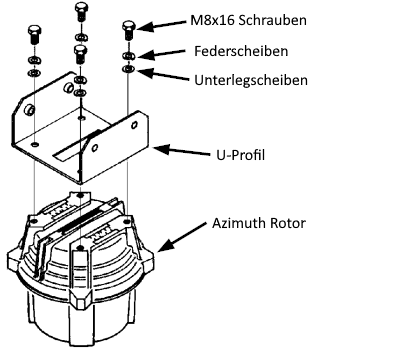
\includegraphics[width=6cm]{../ref/RotorInstallationAzimut.png}
	\label{fig:Rotor_Installation_Azimut_U-Bracket}
	\caption{Azimut Rotor mit U-Profil verbinden}
\end{figure}

\begin{figure}[H]
	\cite{noauthor_yaesu_nodate}
	\centering
	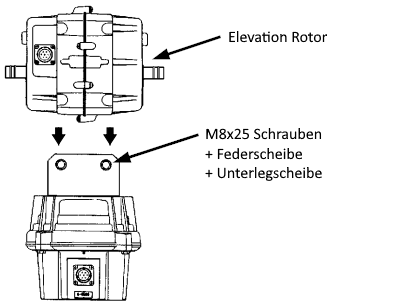
\includegraphics[width=6cm]{../ref/RotorInstallationElevation.png}
	\label{fig:Rotor_Installation_Elevation_U-Bracket+Azimut}
	\caption{Elevation Rotor mit U-Profil und Azimut Rotor verbinden}
\end{figure}



\subsubsection{Kontrollkabel vorbereiten und anschließen}
Für die Ansteuerung der Rotoren werden diese jeweils mit einem 7-Pol-Rundsteckverbinder zum Controller verbunden, wovon 5 Pole verwendet werden. Die Funktion der einzelnen Pins wird im Datenblatt \cite{noauthor_yaesu_nodate} nicht näher beschrieben, konnte allerdings durch Messungen wie folgt bestimmt werden:

Tabelle unbedingt überarbeiten!!!
\newline
\begin{tabular}{| c | l | l |}
	\hline
	\textbf{Pin} & \textbf{Elevation-Funktion} & \textbf{Azimut-Funktion} \\
	\hline
	1 & \multicolumn{2}{| c |}{analoger Ausgang (5V)} \\
	\hline
	2 & \multicolumn{2}{| c |}{analoger Input (0V bis 5V)} \\
	\hline
	3 & \multicolumn{2}{| c |}{analoge Masse} \\
	\hline
	4 & UP Schalter (open collector) & RIGHT Schalter (open collector)\\
	\hline
	5 & DOWN Schalter (open collector) & LEFT Schalter (open collector) \\
	\hline
\end{tabular}

Die Pinbelegung für den 7-Pol-Rundstecker ist im Datenblatt wie folgt angegeben:

\begin{figure}[H]
	\cite{noauthor_yaesu_nodate}
	\centering
	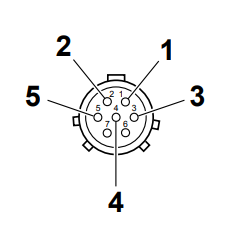
\includegraphics[width=5cm]{../ref/RotorSteckerPinbelegung.png}
	\label{fig:Rotor_Stecker_Pinbelegung}
	\caption{Pinbelegung 7-Pol-Rundstecker (Ansicht vorne)}
\end{figure}

Für die verwendeten Kabel wird im Datenblatt ein Leiterquerschnitt von mindestens 0.5 Quadratmillimeter bei Kabellängen unter 40 Metern und 0.75 Quadratmillimeter bei Kabellängen über 40 Metern vorgeschrieben. Um die Dichtheit der über das Kabel gestülpten Gummikappe zu gewährleisten muss der Außendurchmesser des Kabels zwischen 8.6 bis 10.5 Millimeter betragen.
 
Entsprechend der Pinbelegung im Datenblatt werden die Kabel am anderen Ende mit den Schraubterminal am Rotor Controller verbunden:
\begin{figure}[H]
	\cite{noauthor_yaesu_nodate}
	\centering
	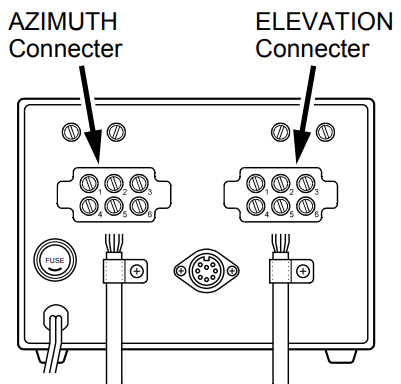
\includegraphics[width=5cm]{../ref/RotorInstallationScrewTerminal.png}
	\label{fig:Rotor_Schraubterminal}
	\caption{Pinbelegung Schraubterminal}
\end{figure}

\subsubsection{Erstinbetriebnahme und kalibrieren der Anzeigen}
Wurden alle Kabel wie beschrieben mit Controller und Rotor verbunden, so kann, nach der Versorgung des Controllers mit Netzspannung, über die DOWN, UP, LEFT und RIGHT Tasten der Rotor manuell bewegt werden. 
\newline
\newline
Für die  Nullkalibrierung wird der Controller ausgeschaltet und die Anzeigenadel über die Schraube auf der Vorderseite unter der jeweiligen Anzeige auf den linken Rand ausgerichtet. Für die Anpassung der Vollaussteuerung der Azimut-Anzeige wird der Controller eingeschalten und der Rotor mithilfe der manuellen Bedientasten bis zum Endschalter nach links gedreht. Die Ausrichtung wird anschließend am Azimut-Rotor, mithilfe von zum Beispiel Klebeband, markiert. Daraufhin wird der Rotor anhand der manuellen Bedientasten nach rechts gedreht, bis er nach einer ganzen Umdrehung wieder den vorher markierten Punkt erreicht. Die Anzeigenadel auf der Azimut-Anzeige sollte sich nun bei 360° befinden, was durch das FULL SCALE ADJ Potentiometer über dem Azimut Schraubterminal auf der Rückseite des Controllers eingestellt werden kann. Für die Kalibrierung des Elevation-Rotor wird dieser mithilfe der manuellen Bedientasten nach oben geschwenkt bis die Ausrichtung genau 180° beträgt. Die Anzeigenadel auf der Elevation-Anzeige sollte sich nun auch bei 180° befinden, was durch das FULL SCALE ADJ Potentiometer über dem Elevation Schraubterminal auf der Rückseite des Controllers eingestellt werden kann.

\subsection {Azimut und Elevation bestimmen}
Die Bestimmung der aktuellen Ausrichtung des Rotors erfolgt über einen von der Rotation des Rotors abhängigen Potentiometer welcher die von Pin 1 zur Verfügung gestellte Spannung teilt. Je nach Ausrichtung ändert sich somit die Spannung am Schleifer des Potentiometers welcher mit Pin 2 verbunden ist. Die Spannung an Pin 2 entspricht somit proportional der Ausrichtung des jeweiligen Rotors. Diese Tatsache wurde durch messtechnische Untersuchungen festgestellt.

